
\documentclass{article}
\usepackage[utf8]{inputenc}
\usepackage{amsmath}

\usepackage{algorithm}
\usepackage{algorithmic}


\usepackage[english]{babel}
\usepackage[T1]{fontenc}
\usepackage{amsmath}
\usepackage{amsfonts}
\usepackage{amssymb}
\usepackage{csvsimple}





\usepackage{graphicx}


\newcommand{\vect}[1]{\ensuremath{\boldsymbol{\mathbf{#1}}}} 
\newcommand{\matr}[1]{\ensuremath{\boldsymbol{\mathbf{#1}}}}

\newcommand{\codevar}[1]{\textbf{#1}}



\usepackage{mathtools}
\DeclarePairedDelimiter\ceil{\lceil}{\rceil}
\DeclarePairedDelimiter\floor{\lfloor}{\rfloor}


\title{Exercise 3 - Spatial Statistics}
\author{Amir Ahmed}
\date{April 2020}


\begin{document}
	\maketitle
	
	\section*{Problem 1: Markov RF}
	Assume that we have observed seismic data over a domain $D \in \mathbb{R}^2$. We want to identify the underlying lithology distribution over D, the underlying lithology of a point is either sand or shale, $\lbrace 1, 0 \rbrace$ respectively.
	
	The observations have been collected on a regular $(75 \times 75)$ grid $L_d$, with seismic data being $\lbrace d(\vect x); \vect x \in L_d \rbrace$. Where $d(\vect x) \in \mathbb{R}$. 
	
	We have observed the lithology distribution in a geologically comparable domain $D_c \in \mathbb{R}^2$. Assume that this was collected on a regular $(66 \times 66)$ grid $L_{D_c}$. 
	
	We assume that the underlying lithology distribution can be represented by a Mosaic RF $\lbrace l(\vect x); \vect x \in  L_D\rbrace, l(\vect x) \in \lbrace 0, 1 \rbrace$.  
	
	
	\subsection*{Problem 1a)}
	 We start by looking at $L_d$.
	 Let the seismic data collection procedure follow the following likelihood model: 
	 $$\left[d_i | \vect l \right] = \begin{cases}
	 0.02 + U_i \text{ if sand, } l_i = 0 \\
	 0.08 + U_i \text{ if shale, } l_i = 1
	 \end{cases}$$
	 $i = 1, 2, \dots, n$. With $U_i$ being identically independently distributed $U_i \sim N(0, 0.06^2)$. This would make each observation point $d_i$ conditionally independent on $\vect l$. That will say: 
	\begin{equation}
		p(d_i | \vect l) = p(d_i | l_i) = \phi(d_i |\mu = 0.02 + 0.06l_i, \sigma^2 = 0.06^2)
	\end{equation}	
	 Where $\phi$ is the pdf of the normal distribution. As all observations are independent we thus have: 
	 \begin{equation}\label{eq:cond_prob}
	 	p(\vect d | \vect l) = \prod_{i=1}^{n}p(d_i | l_i) = \prod_{i=1}^{n}  \phi(d_i |\mu = 0.02 + 0.06l_i, \sigma^2 = 0.06^2)
	 \end{equation} 
	 
	 \begin{figure}[H]	
	 	\begin{center} 
	 		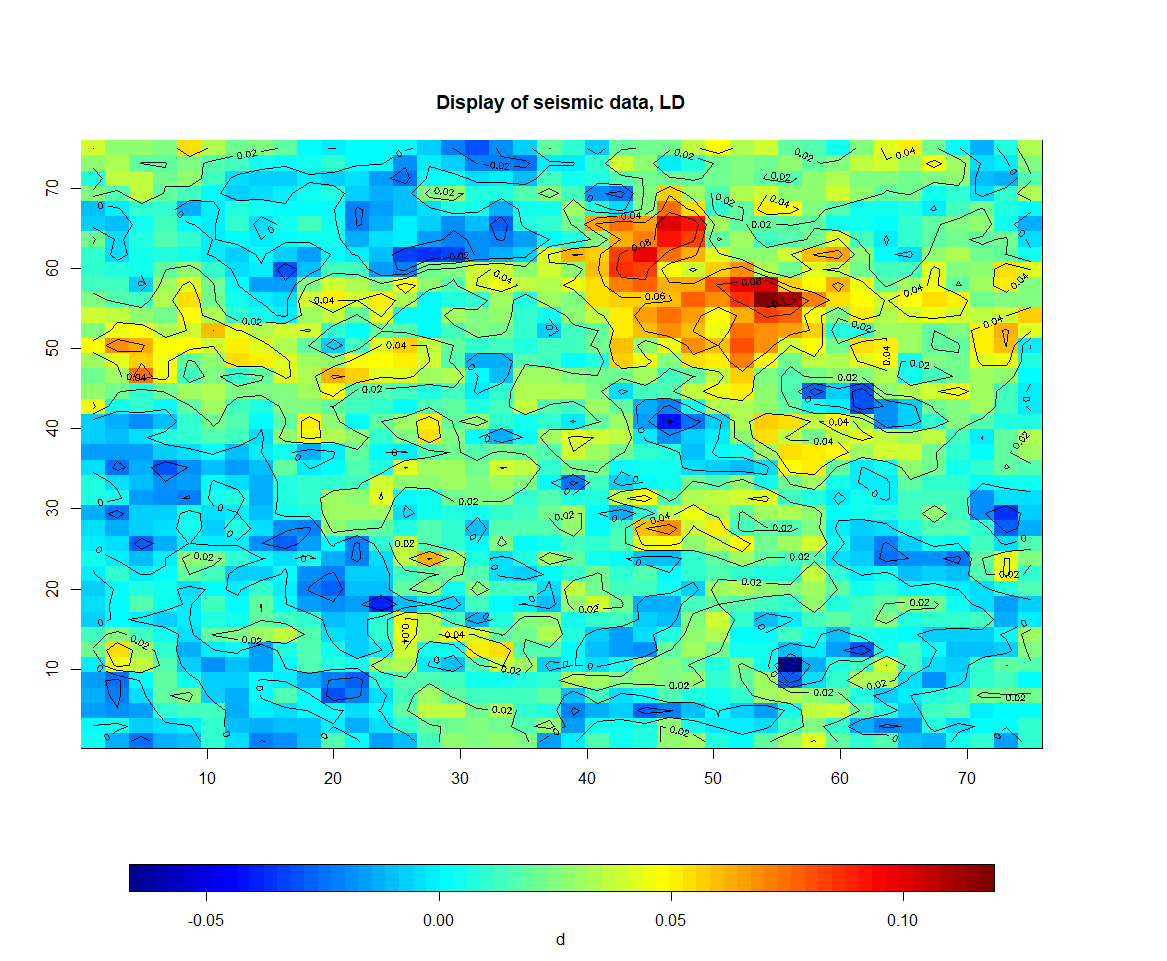
\includegraphics[scale=0.45]{figure1.png}
	 	\end{center}
	 	\caption{Display of seismic data $L_D$.}
	 	\label{fig:1a1} 
	\end{figure}
	 
	 
	 We display the observations from $L_D$ as a map in Figure \ref{fig:1a1}, there seems to be one large gathering where $d(\vect x)$ takes on relatively large values, there also seems to be some smaller gatherings of large $d(\vect x)$ in areas centered around the large one.  

	\newpage
	\subsection*{Problem 1b)}
	We now consider a uniform, independence prior model on $\vect l$. That will say: 
	\begin{equation}
		p(\vect l) = const
	\end{equation}
	We note that since the prior is constant we have:
	\begin{equation}
		p(\vect l | \vect d) \propto p(\vect d | \vect l)
	\end{equation}

	We get the following posterior model using bayes law and the law of total probability: 
	\begin{equation}
		p(\vect l | \vect d) = \dfrac{p(\vect d | \vect l)}{\sum_{\vect l \in \mathbb{L}^n}p(\vect d | \vect l)}
	\end{equation}
	Inserting from \eqref{eq:cond_prob} we get:
	\begin{equation}
		p(\vect l | \vect d) = \dfrac{ \prod_{i=1}^{n}  \phi(d_i |\mu = 0.02 + 0.06l_i, \sigma^2 = 0.06^2)}{\sum_{\vect l' \in \mathbb{L}^n} \prod_{i=1}^{n}  \phi(d_i |\mu = 0.02 + 0.06l_i', \sigma^2 = 0.06^2)}
	\end{equation}
	
	Where $\mathbb{L}^n$ is the n-dimensional space representing all possible values which $l$ can take. 

	As the prior is independent each point would also be conditional independent, for each point we thus get the following. Let: 
	\begin{equation}
		\begin{split}
		p_i &= p(l_i = 1 | d_i) 
		\\ &= \dfrac{p(d_i | l_i = 1)}{p(d_i | l_i = 0) + p(d_i | l_i = 1)}
		\\ &= \dfrac{\phi(d_i |\mu = 0.08, \sigma^2 = 0.06^2)}{\phi(d_i |\mu = 0.02, \sigma^2 = 0.06^2) + \phi(d_i |\mu = 0.08, \sigma^2 = 0.06^2)}
		\end{split}
	\end{equation}
	As each point either is sand or shale we get:
	\begin{equation}
		1 - p_i = p(l_i = 0 | d_i)
	\end{equation}
	We recognize this conditioned model as something Bernoulli-distributed with probability $p_i$. 
	
	We thus have: 
	\begin{equation}
		E(l_i | d_i) = p_i
	\end{equation}
	and 
	\begin{equation}
		Var(l_i | d_i) = p_i(1-p_i)
	\end{equation}
	
	\begin{figure}[H]	
		\begin{center} 
			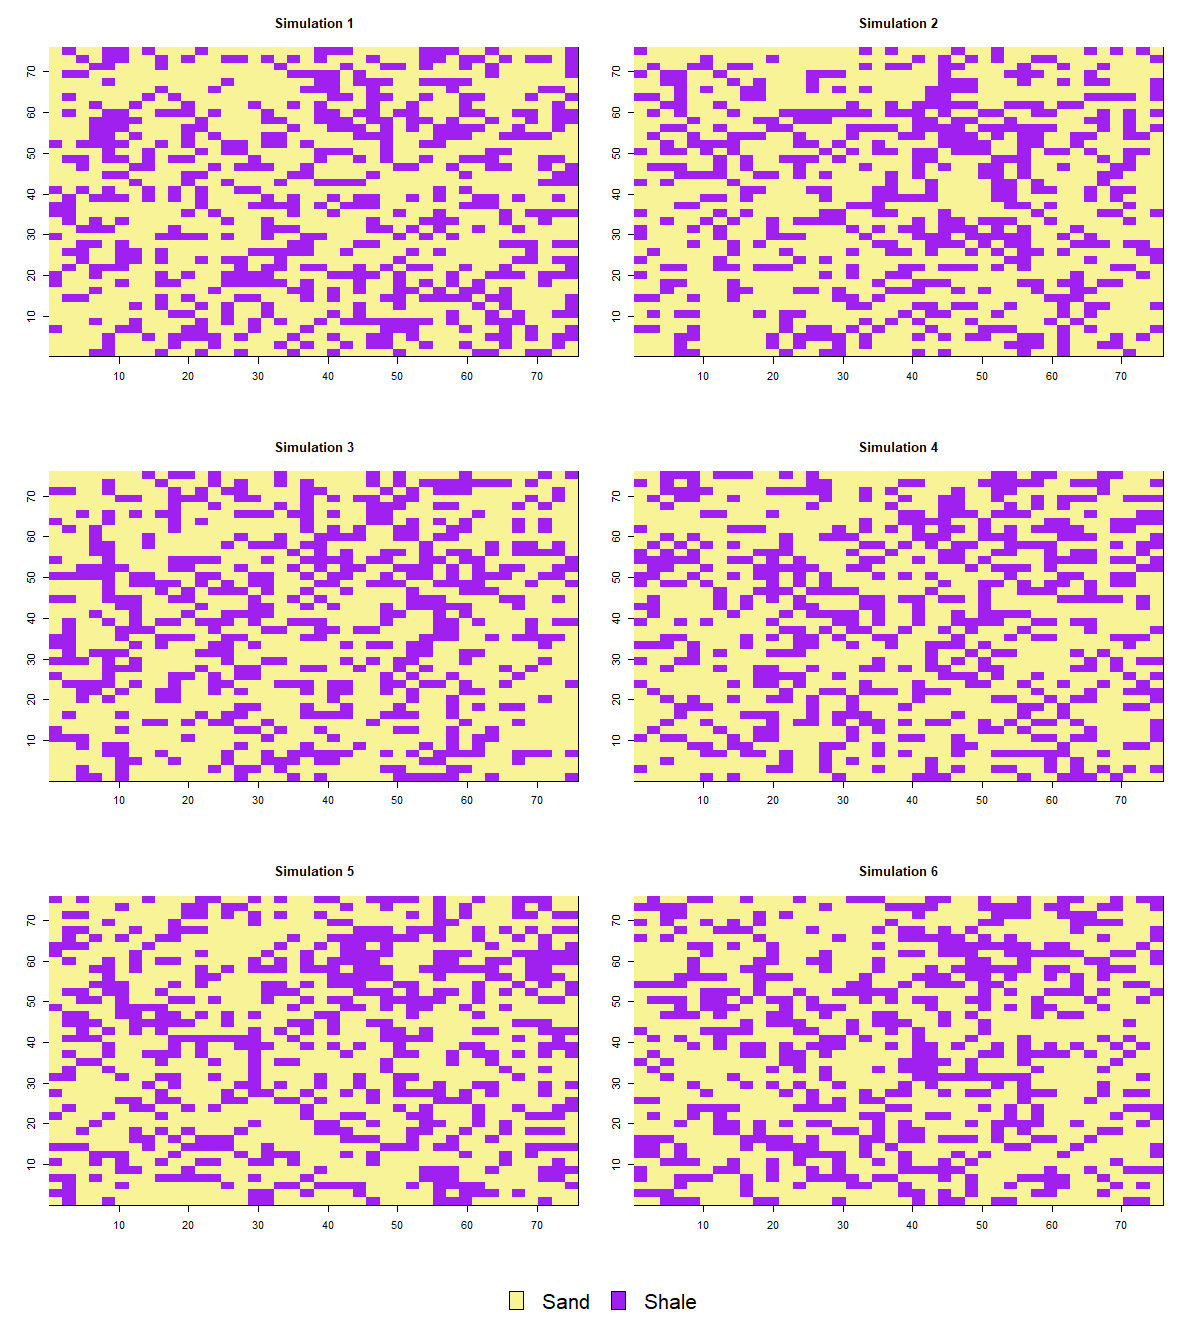
\includegraphics[scale=0.48]{figure2.png}
		\end{center}
		\caption{Display of six posterior realizations of $L_D$.}
		\label{fig:1b1} 
	\end{figure}
	
	
	We simulate 6 trials with the data and display the results in Figure \ref{fig:1b1}. 
	
	The maximum marginal posterior predictor ($MMAP\lbrace \vect l | \vect d \rbrace$) is defined as: 
	\begin{equation}
		MMAP\lbrace \vect l | \vect d \rbrace = \vect{\hat l} = argmax_{\vect l \in \mathbb{L}^n}\lbrace p(\vect l | \vect d)\rbrace
	\end{equation}
	
	Due to the conditional independence of the points we see: 
	\begin{equation}
		\hat l_i = \begin{cases}
		0, \text{ if } p_i < 0.5 \\
		0, \text{ if } p_i \geq 0.5
		\end{cases}
	\end{equation}
	Is a MMAP solution. 
		\begin{figure}[h]	
		\begin{center} 
			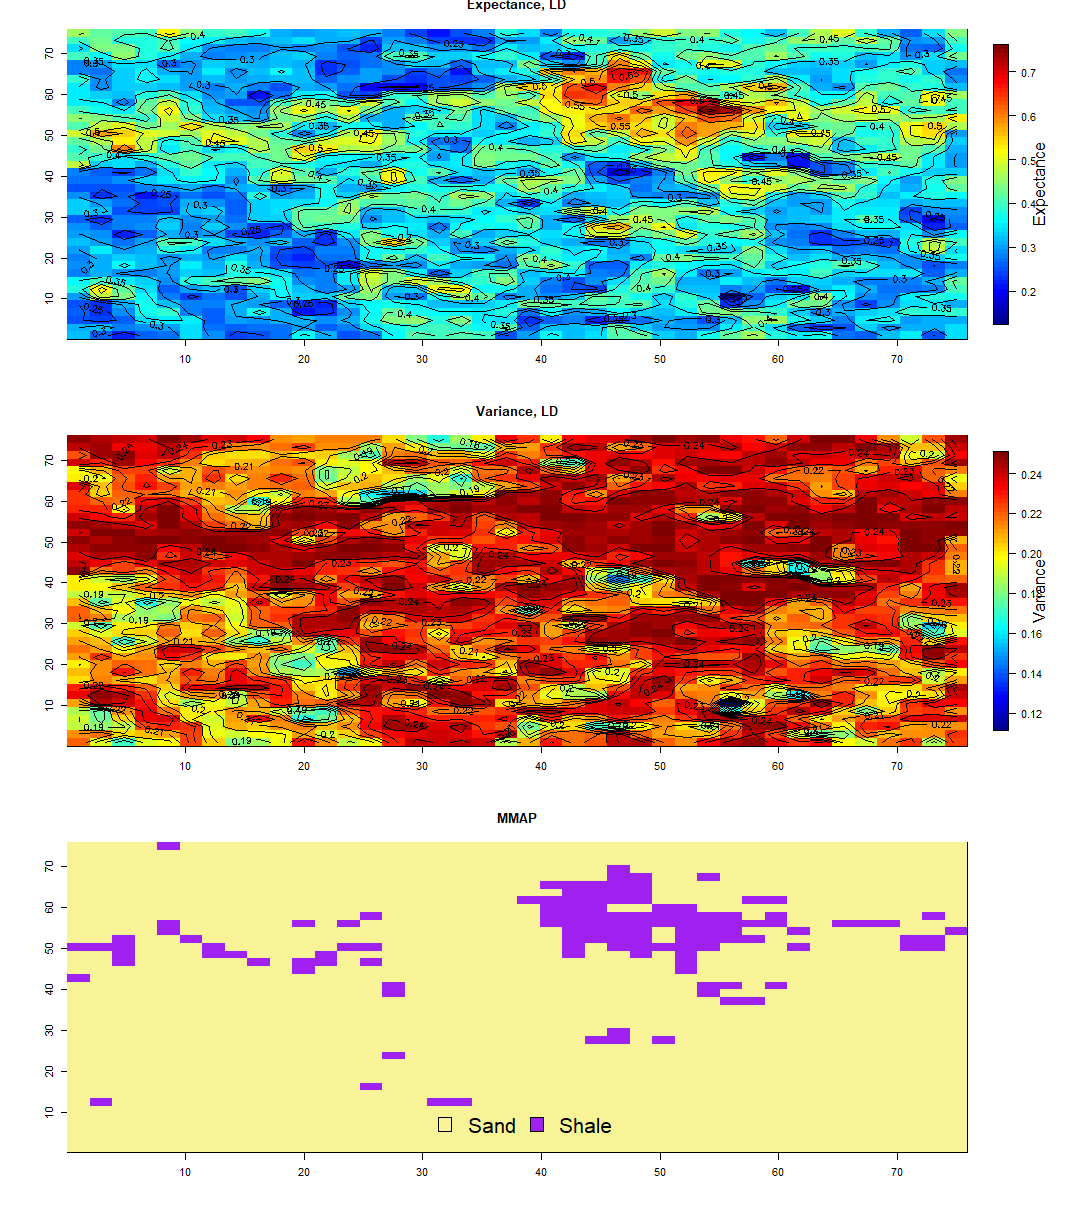
\includegraphics[scale=0.48]{figure4.png}
		\end{center}
		\caption{Display of six posterior realizations of $L_D$.}
		\label{fig:1b2} 
	\end{figure}
	
	We plot MMAP solution, expectance and variance in Figure \ref{fig:1b2}. We see that there is relatively high variance is most parts of the map, this is reflected in the large difference we see between the simulations. From both the expected value and the $MMAP$ we see that there is one large spot (top-right) where we expect a large cluster of shale as with some bands of shale on mid-left. This is somewhat reflected in the simulations. A difference betweeen MMAP and the simulations is that the simulations tend to expect more shale than the MMAP. The map of the expected values seems to be closer to the simulations than the MMAP. 
	
	\pagebreak
	\subsection*{Problem 1c)}
	Now consider a Markov RF prior model for $\lbrace l(\vect x); \vect x \in L_D \rbrace$. Represented by the n-vector $\vect l$ with the clique system $\vect c_L$ consisting of two closest neighbors on the grid $L_D$. 
	
	The corresponding Gibbs formulation is:
	\begin{equation}
		\begin{split}
		p(\vect l) = const \times \prod_{\vect c \in \vect c_L} v_{1l}(l_i, i \in \vect c) &= const \times \prod_{<i, j>\in L_D} \beta^{I(l_i = l_j)} \\
		&= const \times \beta^{\sum_{<i, j>\in L_D} I(l_i = l_j)}
		\end{split}
	\end{equation}
	With $<i, j> \in L_d$ defining the set of two closest neighbors on the grid $L_D$. 
	
	Want to find expressions for the posterior models and want to specify the Markov formulation for the Markov RF. 
	
	Want to find the Markov formulation for the Markov RF. First see:  
	\begin{equation}
		p(l_i | \vect l_{-i}) = \dfrac{p(\vect l)}{\sum_{l_i' \in \mathbb{L}} p(l_i', \vect l_{-i})} = \dfrac{p(\vect l)}{p(l_i = 1, \vect l_{-i}) +p(l_i = 0, \vect l_{-i})} 
 	\end{equation}
 	\begin{equation}
 		p(l_i | \vect l_{-i}) = p(l_i | l_j, j \in n_i)
 	\end{equation}
	
	We note that the joint distribution is given by:
	\begin{equation}
		\begin{split}
				p(\vect d, \vect l) &= p(\vect d | \vect l)p(\vect l) 
				\\ &= const \times \prod_{i=1}^{n}p(d_i | l_i) \prod_{\vect c \in \vect c_L} v_{1l}(l_i, i \in \vect c)
				\\ &= const \times \prod_{i=1}^{n}  \phi(d_i |\mu = 0.02 + 0.06l_i, \sigma^2 = 0.06^2) \prod_{<i, j>\in L_D} \beta^{I(l_i = l_j)}
		\end{split}
	\end{equation}
	
	We input the above into the following:
	\begin{equation}
		p(\vect l | \vect d) = \dfrac{p(\vect l, \vect d)}{p(\vect d)} = const  \times \prod_{i=1}^{n}  \phi(d_i |\mu = 0.02 + 0.06l_i, \sigma^2 = 0.06^2) \prod_{<i, j>\in L_D} \beta^{I(l_i = l_j)}
	\end{equation}
	Also: 
	\begin{equation}
	\begin{split}
		p(l_i, \vect d | \vect l_{-i}) &= p(\vect d | \vect l)p(l_i | \vect l_{-i}) \\ &= p(\vect d | \vect l)p(l_i | \vect l_{-i}) \\ 
		&= 	\dfrac{p(\vect l)}{p(l_i = 1, \vect l_{-i}) +p(l_i = 0, \vect l_{-i})} 	\prod_{i=1}^{n}  \phi(d_i |\mu = 0.02 + 0.06l_i, \sigma^2 = 0.06^2) 
	\end{split}
	\end{equation}
	Let $n_i$ be the neighborhood around the ith node. Then have:
	\begin{equation}
		p(l_i, \vect d | \vect l_{-i}) = \dfrac{\prod_{<i, j> \in n_i}\beta^{I(l_i = l_j)}}{\prod_{<i, j> \in n_i}\beta^{I(0 = l_j)} + \prod_{<i, j> \in n_i}\beta^{I(1 = l_j)}} 	\prod_{i=1}^{n}  \phi(d_i |\mu = 0.02 + 0.06l_i, \sigma^2 = 0.06^2) 
	\end{equation} 
	as the Markov formulation. 
	
	Now want to develop expressions for the posterior model  $p(l_i | \vect d, \vect l_{-i})$ have:
	\begin{equation}
		\begin{split}
		p(l_i | \vect d, \vect l_{-i}) &= p(l_i | d_i, l_{j}, j \in n_i) 
		\\ &= \dfrac{p(d_i | l_i)\prod_{<i, j> \in n_i}\beta^{I(l_i = l_j)}}{\phi(d_i|\mu = 0.02, \sigma^2 = 0.06^2)\prod_{<i, j> \in n_i}\beta^{I(l_j = 0)} + \phi(d_i|\mu = 0.08, \sigma^2 = 0.06^2)\prod_{<i, j> \in n_i}\beta^{I(l_j = 1)}} 
		\end{split}		
	\end{equation} 
	
	We now display the observations in $D_c$
\end{document}